\chapter{Data and Methods}

The differentiation of crop types in remotely-sensed imagery is not a straightforward process. The use of a vegetation index (VI), such as the normalized difference vegetation index (NDVI) or the enhanced vegetation index (EVI), can help identify crops by their specific VI values in an image.

NDVI is a normalized ratio of the red and near-infrared bands, and can be expressed mathematically as:
\begin{equation}
  NDVI = \frac{\rho~_{NIR} - \rho~_{red}}{\rho~_{NIR} + \rho~_{red}}
\end{equation}
where $\rho~_{NIR}$ and $\rho~_{red}$ are the measured surface reflectance in their respective bands. As a ratio, the index minimizes multiplicative noise, but has issues with non-linearity and additive noise \autocite{huete2002overview}.

With advances in calibration, atmospheric correction, and other noise removal techniques which are integrated into the MODIS data processing workflow, a ratioing index is less necessary. The EVI was specifically developed for the MODIS platform to help correct some of the deficiencies of the NDVI. It has better sensitivity to high biomass, canopy structure, and leaf area, and less susceptibility to atmospheric degradation. EVI is calculated as:
\begin{equation}
  EVI = G\frac{\rho~_{NIR} - \rho~_{red}}{\rho~_{NIR} +  C_1\times\rho~_{red} - C_2 \times \rho~_{blue} + L}
\end{equation}
Again, each $\rho$ is the measured surface reflectance in the respective band, after complete or partial atmospheric correction. The blue band is used to "subtract" aerosol effects from the red band. Additionally, four coefficients are introduced: $G$ is the gain factor, $C_1$ and $C_2$ are used in the aerosol calculation, while $L$ "is the canopy background adjustment that addresses nonlinear, differential NIR and red radiant transfer through a canopy" \citereset\autocite[196]{huete2002overview}. The values of these coefficients as used in the MODIS EVI calculation are 2.5, 6.0, 7.5, and 1.0, respectively.

Some crops, such as soy and sugarcane, have very different spectral reflectance throughout their development and maturation, however others, such as soy and corn, can have very similar reflective curves, leading to overlapping VI ranges. Such overlap can make it impossible to determine a crop type with specificity using traditional approaches. To combat this, a time series of images can be used to find VI values throughout a year to develop a classification based on annual phenology rather than a single-date image \autocites{gu2010phenological}{wardlow2002discriminating}{wardlow2005state-level}{wardlow2007analysis}{wardlow2008large-area}{zhang2003monitoring}.
	
In this study, I will use 16-day MODIS NDVI and EVI composite images to perform the phenological VI classification. One specific advantage of MODIS data is its temporal resolution; as the satellite passes any given location on a daily basis, the likelihood of getting enough cloud-free data to develop a phenologic model is significantly increased over other common platforms like Landsat Thematic Mapper (TM) and Landsat Operational Land Imager (OLI), which only have repeat coverage every sixteen days. MODIS data, however, comes at the price of a reduced spatial resolution of 250 meters compared to Landsat’s 30-meter pixels.

Each of the 16-day composite VI images will be used as a band in a multi-date time-series image representing an entire agricultural year. The images are numbered by the day of the year (DOY) of the last date in the image, so an image from DOY 17 is the composite of the images from January 2 through January 17. In Kansas, an entire agricultural year can be captured from January 2 through the following January 1. Therefore, a Kansas time-series image with 16-day composite imagery would require 23 bands, band one being the composite image from January 17, with each succeeding band progressing every sixteen days through the end of the year (thus band 2 is DOY 33, band 3 is DOY 49, band 4 is DOY 65, etc.). Technically, following this pattern will make the last band of the image be from January 4 the following year, but the MODIS composite numbering "resets" at the end of each year, and band 23 ends up being from January 1.

In Argentina, as it is in the Southern Hemisphere and the seasons are inverted to those of the Northern hemisphere, the growing season shifts, as must the date range for the VI time-series in order to capture crop phenologies unbroken. That is, the time-series image for Pellegrini must begin mid-calendar-year to adequately capture the annual phenologies. To accomplish this, the time-series images begin with the 16-day composite image from DOY 193 (July 12 in common years) and end with the image from the following DOY 177 (June 26 in common years).

\citeauthor{gu2010phenological} outlined that phenological statistics regarding vegetation development can be derived from a MODIS VI time-series, including “start-of-season time (SOST), start-of-season NDVI (SOSN), end-of-season time (EOST), end-of-season NDVI (EOSN), maximum NDVI (MAXN), maximum NDVI time (MAXT), duration of season (DUR), amplitude of NDVI (AMP), and seasonal time integrated NDVI (TIN)” \mkbibparens{\citeyear[529]{gu2010phenological}}. A principal component analysis (PCA) can then be used to extract the meaningful variation in the data. Similarly, Wardlow, Egbert, et al. \autocites{wardlow2002discriminating}{wardlow2005state-level}{wardlow2007analysis}{wardlow2008large-area} showed that a decision tree classifier can be used to classify vegetation time-series data into increasingly refined categories until specific crop types are isolated and classified. By beginning with a basic land cover classification (e.g. forest, urban, agriculture), crops in the agriculture class can be broken down into winter and summer varieties using peaks in the vegetation index (winter wheat will peak earlier in the year than summer crops like corn and soy). Then, using training sites of known crop types defined by ground truth data, a final crop classification can be assigned by finding pixel values for key dates where like crops can be differentiated. That is, using the growing season in the Northern Hemisphere as an example, if from the training sites we know crop A has VI values between 0.7 and 0.8 on June 26 and between 0.5 and 0.6 on August 29, while crop B is between 0.55 and 0.65 and 0.75 and 0.85 on the same dates, pixels in the summer crop class can be assigned one of these types by testing their pixel values on these dates. While the authors found this method to have about an 85 percent overall accuracy \autocite{wardlow2005state-level}, the downside of this method is that it requires training sites with previously-determined crop types to produce a classification, which can be time consuming and expensive to acquire.

\textcite{masialeti2010a-comparative} found that VI values from one year have a significant correlation with values from other years. Comparing the phenological curves of crops formed by the NDVI values from 2001 MODIS data \autocite[from][]{wardlow2005state-level} with those from 2005 MODIS data, the authors found the overall shape of each crop's curve is maintained year-to-year, with subtle shifts in the beginning of the curve (earlier or later planting), the maximum of the curve, and the spread of the curve (a longer or shorter growing season), depending on weather and other external variables (Fig. \ref{fig:transformations}). They surmised, with a means to account for these shifts of the curve, one could use VI values from one year to classify those from another.

\begin{figure}
  \centering
  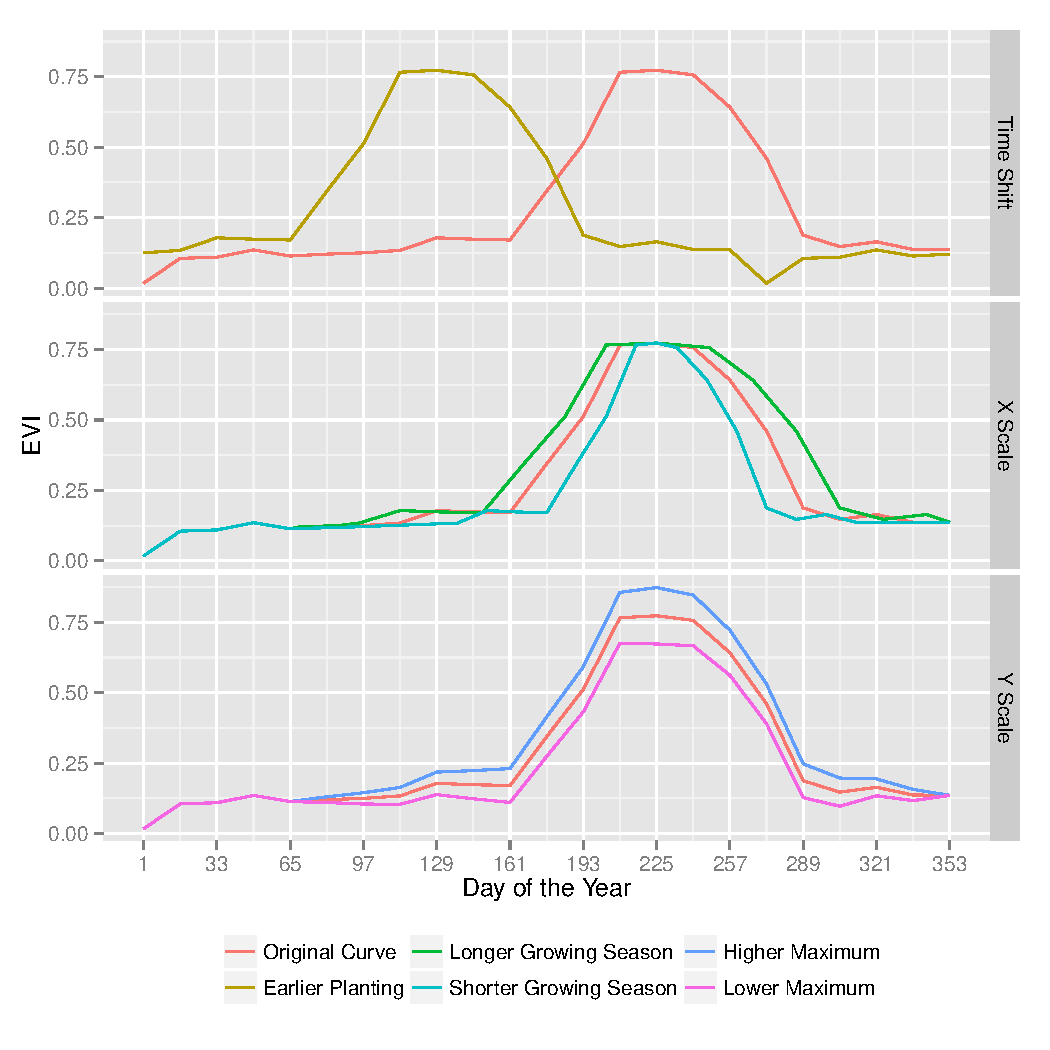
\includegraphics[width=\textwidth]{Graphics/transformations.pdf}
  \caption{Examples of transformations of a crop's VI curve due to interannual variations in growing conditions. The original curve is that found for soy in the initial test area (see the Preliminary Results on pg. \pageref{sec:prelim}). The other curves were arbitrarily adjusted to illustrate each of the possible transformations.}
  \label{fig:transformations}
\end{figure}

\textcites{sakamoto2005a-crop}{sakamoto2010a-two-step} has shown that MODIS time-series data can be used to find key dates in a crop’s phenology, enabling better crop management strategies. Specifically, the authors’ two-step filter (TSF) method uses a wavelet transformation and a constrained minimization function to find reference curves for a specific crop’s phenological development, and then fits that curve to known pixels of that crop type to find the transition between developmental stages in the plants’ growth. This TSF method demonstrates that reference curves can be fit to a pixel’s values using a minimization function, accounting for the variations from the reference curve and the pixel curve. Therefore, unlike the previous multi-date VI classification approaches, which require trainings sites, this minimization method could be used without training sites to classify imagery by fitting previously-known references curves (i.e. not derived from ground truth data) to pixel values in a VI time-series; such is the foundation of the method I wish to test.

Drawing extensively from \textcite{sakamoto2010a-two-step}, I am in the process of developing said method. From page 2151:
\begin{equation}
  RMSE = \biggl[\frac{1}{365/s}\sum_{x=d,d+s,d+2s...}^{365}\bigl(f\left(x\right)-g\left(x\right)\bigr)^{2}\biggr]^{\frac{1}{2}}
\end{equation}
where $s$ is the interval of the imagery, $d$ is the starting date of the imagery, $f(x)$ is the phenological curve for a given pixel in a dataset, and $x$ is the DOY. $g(x)$ is given by:
\begin{equation}\label{eq2}
  g(x) = yscale\times~h\left(xscale\times(x_0 + tshift)\right)
\end{equation}

Here, $yscale$ and  $xscale$ are coefficients controlling the vertical and horizontal scaling of a reference curve $h(x_0)$, and $tshift$ is a constant representing the horizontal shift, in days, of $h(x_0)$ (Fig. \ref{fig:transformations}). $x_0$ is the day of year in the shape model. Thus, if we minimize eq. 3 bounding $yscale$, $xscale$, and $tshift$  in $g(x)$ with reasonable values for each, we can calculate how well a given reference curve $h(x_0)$ can be made to fit the pixel values $f(x)$. Comparing the minimum RMSE of each of the reference curves used allows us to assign a confidence score that a pixel is one of the crops we are seeking. Using Bayesian probability theory or Dempster-Shafer theory of evidence, a pixel's confidence score for each of the crop types will determine the final crop classification and uncertainty of the classification \autocite{jiang2000application}.

As this is a new approach to crop classification, a variety of variables need to be tested to see how they impact the resulting classification, including:
%\begin{spacing}{1.2}
\begin{itemize}
  \item The spatial distribution of pixels chosen to create the reference curves.
  \item The temporal distribution of pixels chosen to create the reference curves.
  \item The VI used for the classification.
\end{itemize}
%\end{spacing}
To test these factors, I will iteratively run the analysis using five small sample areas dispersed across Kansas. With the USDA CDL as ground truth reference, I will test the classification in each of the sample areas using reference curves derived from one, two, three, and four of the sample areas, to see if multiple sites being averaged increases the accuracy of the reference curves, or introduces noise due to geographical discrepancies in season start, maximum intensity, or season length. Similarly, I will add multiple years of data to each sample location, to see if averaging curves over those years has a positive or negative effect on the classification results. Lastly, I will perform all of theses tests twice, once with MODIS NDVI data, and again with MODIS EVI data. From this testing, I can determine the best method for deriving crop reference curves, and use the reference curves from that method and apply them to classifying the data from my study area in Argentina.

The accuracy of the Argentina study area classification will need to be assessed, which will require ground truth data to verify whether the classification identified the pixels correctly. Unfortunately, data like the USDA CDL does not exist for Argentina. In order to acquire the necessary ground truth, I will create a set of control points using a stratified random approach. This will provided me with a random sample of points throughout each of the different classes identified (i.e. corn, soy, wheat, not crops). Then, I will visit each of these points to determine the crop cover or land cover. I will use this ground truth data to construct a confusion matrix in order to check the producer, user, and overall accuracies of the classification.